En este capítulo se describe la metodología se trabajo seguida, tanto desde un punto de vista de gestión de proyecto como desde el punto de vista técnico.\\

\section{Scrum}
Durante todo el desarrollo se ha empleado la metodología ágil \textit{Scrum}. Este método se caracteriza porque se realizan entregas parciales y regulares del producto final priorizando aquellas tareas que sean de mayor importancia para el resultado deseado. El desarrollo se ejecuta en ciclos temporales cortos y de duración fija (\textit{Sprints}) y al finalizar deben proporcionar un incremento del producto que sea susceptible de ser entregado. Tras esto, se realiza una reunión con el \textit{Product Owner} para evaluar el resultado \textit{Sprint review} y se planifica la siguiente iteración (\textit{Sprint planning}).\\

\begin{figure}[h]
\centering
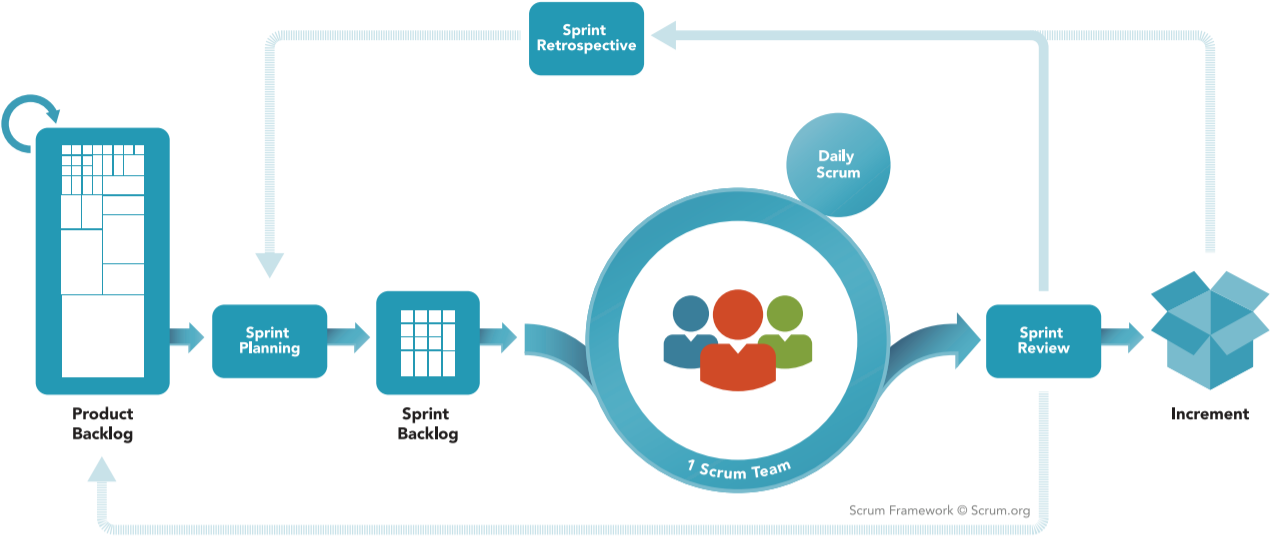
\includegraphics[scale=0.4]{../images/scrum.png} 
\caption{Metodología Scrum. Fuente: scrum.org/resources/scaling-scrum}
\label{fig:x scrum}
\end{figure}

Dada la naturaleza del proyecto y la poca experiencia previa en el desarrollo de chatbots esta forma de trabajar aporta la suficiente flexibilidad para subsanar los posibles errores o problemas que surjan durante el proceso de diseño o desarrollo. Por otra lado, una parte crucial en la construcción de cualquier chatbot es poder empezar a probar el servicio con usuarios reales cuando antes, de manera que se pueda ir incorporando a la base de datos toda la información recopilada y el desarrollo se pueda beneficiar de este \textit{feedback}. Es en este punto donde la entrega de valor en períodos cortos de tiempo de \textit{Scrum} es idónea para el proyecto, ya que estas iteraciones posibilitan tener una producto mínimo viable (\textit{PMI}) cuanto antes.\\

En este proyecto los \textit{Sprints} han sido de 2 semanas naturales de duración, realizando el día 14 una reunión con el \textit{Product Owner} (los tutores del proyecto) para valorar el progreso realizado y determinar las próximos pasos a seguir. \\

Por otra parte, también se ha mantenido un contacto constante a través de reuniones \textit{online} y correos electrónicos con los investigadores del Hospital General de Elche para contar en todo momento con su visto bueno en temas médicos y de diseño.\\

En los documentos anexos a este trabajo se pueden encontrar las actas de todas estas reuniones con la fecha, los participantes y los temas tratados.\\

\section{Control de versiones}
Durante el desarrollo se ha utilizado \textit{Git} como herramienta de control versiones, manteniendo así un control sobre los cambios realizados en el código. Se trabajó con dos repositorios, uno para el \textit{frontend} \cite{gitApp} y otro para el \textit{backend} \cite{gitChatbot} (ver sección \ref{arquitectura}), ambos con 2 ramas distintas: \textit{master} y \textit{develop}. Durante el trascurso del \textit{sprint} se trabajaba sobre \textit{develop} y en una máquina local. Al finalizar, si todo funcionaba correctamente, se realizaba un \textit{merge} a \textit{master} para incorporar a la rama estable los últimos cambios.\\

Esta metodología de trabajo era crucial, ya que, durante una gran parte del desarrollo se tuvo a disposición un servidor de producción donde funcionaba el chatbot (ver sección \ref{despliegue}). Este servidor estaba siempre actualizado con la última versión de la rama \textit{master}, y por tanto, era muy importante que fuera lo más estable posible.\\

\section{Roadmap}
\label{roadmap}
Siguiendo la metodología \textit{Scrum} se propone una ruta de desarrollo (ver Figura \ref{fig:roadmap desarrollo}) centrada en la obtención de un producto mínimo viable lo antes posible. Para ello primeramente se realizan los diseños del chatbot, se organiza la información recibida y se trabaja para la obtención de un \textit{PMI} en versión web. A partir de ese punto es se publica una versión de prueba del \textit{bot} para empezar con la obtención de datos reales  y realizar distintas iteraciones sobre el producto hasta conseguir el resultado deseado. Una vez se alcanza el nivel de madurez requerido, la web se empaqueta como \textit{app} para móvil y se publica.\\

\begin{figure}[htbp]
\centering
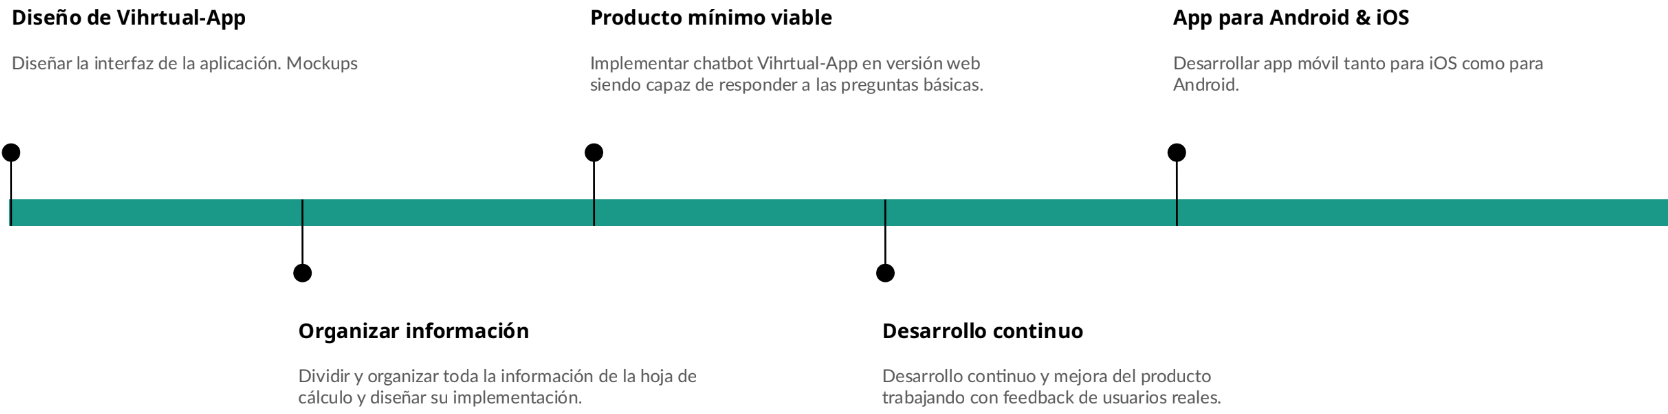
\includegraphics[scale=0.4]{../images/roadmap.png} 
\caption{\textit{Roadmap} propuesto para el desarrollo de VIHrtual-App}
\label{fig:roadmap desarrollo}
\end{figure}


